\documentclass[12pt, aspectratio=169]{beamer}

% ─────────────────────────────────────────────
%  Tema y colores
% ─────────────────────────────────────────────
\usetheme{Madrid}
\usecolortheme{seahorse}

\definecolor{azuloscuro}{RGB}{10, 60, 120}
\definecolor{azulmedio}{RGB}{30, 100, 180}
\definecolor{dorado}{RGB}{204, 153, 0}
\definecolor{verdeclaro}{RGB}{0, 140, 100}
\definecolor{grisclaro}{RGB}{245, 245, 250}

\setbeamercolor{palette primary}{bg=azuloscuro, fg=white}
\setbeamercolor{palette secondary}{bg=azulmedio, fg=white}
\setbeamercolor{palette tertiary}{bg=dorado, fg=white}
\setbeamercolor{palette quaternary}{bg=azuloscuro, fg=white}
\setbeamercolor{structure}{fg=azuloscuro}
\setbeamercolor{block title}{bg=azuloscuro, fg=white}
\setbeamercolor{block body}{bg=grisclaro, fg=black}
\setbeamercolor{block title alerted}{bg=dorado!90!black, fg=white}
\setbeamercolor{block body alerted}{bg=dorado!10, fg=black}
\setbeamercolor{block title example}{bg=verdeclaro, fg=white}
\setbeamercolor{block body example}{bg=verdeclaro!10, fg=black}
\setbeamercolor{frametitle}{bg=azuloscuro, fg=white}
\setbeamercolor{title}{fg=white}
\setbeamercolor{subtitle}{fg=dorado!80!white}

% ─────────────────────────────────────────────
%  Fuentes
% ─────────────────────────────────────────────
\usepackage[T1]{fontenc}
\usepackage[utf8]{inputenc}


\usepackage{amsmath, amssymb, amsthm}
\usepackage{mathtools}
\usepackage{array, booktabs, tabularx}
\usepackage{tikz}
\usetikzlibrary{arrows.meta, shapes.geometric, positioning, decorations.pathreplacing, calc}
\usepackage{pgfplots}
\pgfplotsset{compat=1.18}
\usepackage{xcolor}
\usepackage{tcolorbox}
\tcbuselibrary{theorems, skins, breakable}
\usepackage{enumitem}
\usepackage{multicol}
\usepackage{pifont}

% ─────────────────────────────────────────────
%  Cajas personalizadas
% ─────────────────────────────────────────────
\newtcolorbox{definicion}[1]{
  enhanced, title=#1,
  colback=azuloscuro!5, colframe=azuloscuro,
  fonttitle=\bfseries\small, coltitle=white,
  attach boxed title to top left={yshift=-2mm, xshift=4mm},
  boxed title style={colback=azuloscuro, colframe=azuloscuro},
  top=6pt, left=6pt, right=6pt, bottom=6pt
}

\newtcolorbox{propiedad}[1]{
  enhanced, title=#1,
  colback=azulmedio!8, colframe=azulmedio,
  fonttitle=\bfseries\small, coltitle=white,
  attach boxed title to top left={yshift=-2mm, xshift=4mm},
  boxed title style={colback=azulmedio},
  top=6pt, left=6pt, right=6pt, bottom=6pt
}

\newtcolorbox{ejercicio}[1]{
  enhanced, title=\ding{46}\; #1,
  colback=verdeclaro!8, colframe=verdeclaro,
  fonttitle=\bfseries\small, coltitle=white,
  attach boxed title to top left={yshift=-2mm, xshift=4mm},
  boxed title style={colback=verdeclaro},
  top=6pt, left=6pt, right=6pt, bottom=6pt
}

\newtcolorbox{alerta_box}[1]{
  enhanced, title=!\; #1,
  colback=dorado!10, colframe=dorado!80!black,
  fonttitle=\bfseries\small, coltitle=black,
  attach boxed title to top left={yshift=-2mm, xshift=4mm},
  boxed title style={colback=dorado!80!black, coltitle=white},
  top=6pt, left=6pt, right=6pt, bottom=6pt
}

% ─────────────────────────────────────────────
%  Navegación limpia
% ─────────────────────────────────────────────
\setbeamertemplate{navigation symbols}{}
\setbeamertemplate{footline}{
  \leavevmode
  \hbox{
    \begin{beamercolorbox}[wd=.33\paperwidth, ht=2.5ex, dp=1.125ex, leftskip=.3cm]{palette primary}
      \usebeamerfont{author in head/foot}\insertshortauthor
    \end{beamercolorbox}
    \begin{beamercolorbox}[wd=.34\paperwidth, ht=2.5ex, dp=1.125ex, center]{palette secondary}
      \usebeamerfont{title in head/foot}\insertshorttitle
    \end{beamercolorbox}
    \begin{beamercolorbox}[wd=.33\paperwidth, ht=2.5ex, dp=1.125ex, rightskip=.3cm, right]{palette primary}
      \usebeamerfont{date in head/foot}\insertframenumber{} / \inserttotalframenumber
    \end{beamercolorbox}
  }
  \vskip0pt
}

% ─────────────────────────────────────────────
%  Información del documento
% ─────────────────────────────────────────────
\title[Potencias y Álgebra Real]{\textbf{Potencias y Álgebra en los Números Reales}}
\subtitle{Fundamentos, Propiedades y Patrones Algebraicos}
\author[Matemáticas]{Cátedra de Matemáticas}
\institute[Universidad]{\textit{Departamento de Ciencias Exactas}\\[2pt]\small Cálculo y Álgebra -- Primer Semestre}
\date{\today}

% ─────────────────────────────────────────────
%  DOCUMENTO
% ─────────────────────────────────────────────
\begin{document}

%──────────── PORTADA ────────────────────────
{
\setbeamertemplate{headline}{}
\setbeamertemplate{footline}{}
\begin{frame}
  \begin{tikzpicture}[remember picture, overlay]
    \fill[azuloscuro] (current page.north west) rectangle ([yshift=-0.35\paperheight]current page.north east);
    \fill[dorado] ([yshift=-0.35\paperheight]current page.north west) rectangle ([yshift=-0.38\paperheight]current page.north east);
    \node[anchor=north, text=white, font=\Large\bfseries] at ([yshift=-1.2cm]current page.north) {POTENCIAS Y ÁLGEBRA EN LOS NÚMEROS REALES};
    \node[anchor=north, text=dorado!80!white, font=\normalsize\itshape] at ([yshift=-2.4cm]current page.north) {Fundamentos, Propiedades y Patrones Algebraicos};
    \node[anchor=south east, text=white!70!azuloscuro, font=\small] at ([xshift=-0.5cm, yshift=0.3cm]current page.south east) {Cátedra de Matemáticas · \today};
  \end{tikzpicture}
  \vspace*{4.5cm}
  \begin{columns}[T]
    \column{0.5\textwidth}
    {\color{azuloscuro}\textbf{\large Contenidos de la sesión:}}\\[6pt]
    \small
    \begin{itemize}[leftmargin=*]
      \item[\textcolor{dorado}{$\blacktriangleright$}] Concepto y propiedades de potencias
      \item[\textcolor{dorado}{$\blacktriangleright$}] Álgebra real: términos y expresiones
      \item[\textcolor{dorado}{$\blacktriangleright$}] Términos semejantes y simplificación
      \item[\textcolor{dorado}{$\blacktriangleright$}] Patrones y relaciones algebraicas
    \end{itemize}
    \column{0.45\textwidth}
    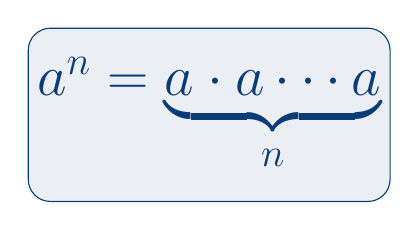
\begin{tikzpicture}[scale=0.85]
      \node[draw=azuloscuro, fill=azuloscuro!8, rounded corners=8pt,
            minimum width=4cm, minimum height=2.2cm,
            font=\huge\bfseries, text=azuloscuro] at (0,0)
            {$a^n = \underbrace{a \cdot a \cdots a}_{n}$};
    \end{tikzpicture}
  \end{columns}
\end{frame}
}

%──────────── ÍNDICE ─────────────────────────
\begin{frame}{Tabla de Contenidos}
  \begin{columns}
    \column{0.5\textwidth}
    \tableofcontents[sections={1-2}]
    \column{0.5\textwidth}
    \tableofcontents[sections={3-4}]
  \end{columns}
\end{frame}

% ═══════════════════════════════════════════════
\section{Concepto de Potencia}
% ═══════════════════════════════════════════════

\begin{frame}{¿Qué es una Potencia?}
  \begin{columns}[T]
    \column{0.52\textwidth}
    \begin{definicion}{Definición Formal}
      Sea $a \in \mathbb{R}$ y $n \in \mathbb{N}$. Se define la \textbf{potencia} de base $a$ y exponente $n$ como:
      \[
        a^n \;=\; \underbrace{a \cdot a \cdot \ldots \cdot a}_{n \text{ factores}}, \quad n \geq 1
      \]
      Con la convención: $a^0 = 1$ para $a \neq 0$.
    \end{definicion}
    \vspace{6pt}
    \begin{alerta_box}{Caso especial: $0^0$}
      La expresión $0^0$ es una \textbf{indeterminación} en análisis matemático, aunque en combinatoria se adopta el convenio $0^0 = 1$.
    \end{alerta_box}

    \column{0.44\textwidth}
    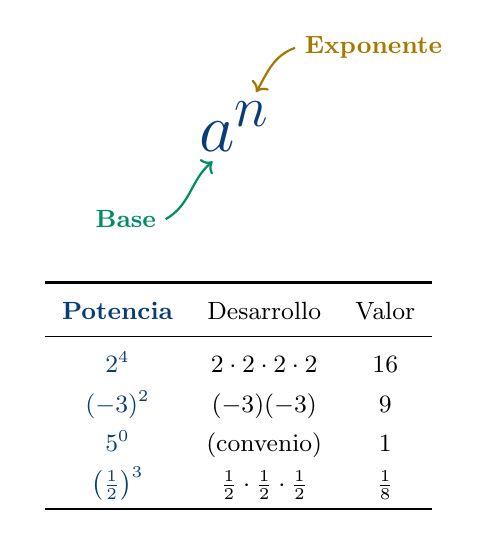
\begin{tikzpicture}[scale=0.92]
      % Diagrama base-exponente
      \node[font=\Huge\bfseries, text=azuloscuro] (expr) at (0,0) {$a^n$};
      \node[font=\small, text=verdeclaro, below left=0.5cm and 0.3cm of expr] (base) {\textbf{Base}};
      \node[font=\small, text=dorado!80!black, above right=0.3cm and 0.2cm of expr] (exp) {\textbf{Exponente}};
      \draw[->, verdeclaro, thick] (base.east) to[out=30, in=220] ([xshift=-0.3cm]expr.south);
      \draw[->, dorado!80!black, thick] (exp.west) to[out=200, in=60] ([xshift=0.3cm]expr.north);

      % Tabla de ejemplos
      \node[below=1.4cm of expr, font=\small] {
        \renewcommand{\arraystretch}{1.3}
        \begin{tabular}{>{\color{azuloscuro}\bfseries}c c c}
          \toprule
          Potencia & Desarrollo & Valor \\
          \midrule
          $2^4$ & $2\cdot2\cdot2\cdot2$ & $16$ \\
          $(-3)^2$ & $(-3)(-3)$ & $9$ \\
          $5^0$ & (convenio) & $1$ \\
          $\left(\tfrac{1}{2}\right)^3$ & $\tfrac{1}{2}\cdot\tfrac{1}{2}\cdot\tfrac{1}{2}$ & $\tfrac{1}{8}$ \\
          \bottomrule
        \end{tabular}
      };
    \end{tikzpicture}
  \end{columns}
\end{frame}

\begin{frame}{Extensión: Exponentes Enteros Negativos}
  \begin{columns}[T]
    \column{0.48\textwidth}
    \begin{definicion}{Exponente Negativo}
      Para $a \neq 0$ y $n \in \mathbb{N}$:
      \[
        a^{-n} \;=\; \frac{1}{a^n}
      \]
    \end{definicion}
    \vspace{4pt}
    \begin{block}{Motivación desde el patrón}
      Observa la siguiente secuencia:
      \medskip

      \renewcommand{\arraystretch}{1.4}
      \begin{tabular}{cc}
        \toprule
        Potencia & Valor \\
        \midrule
        $2^3$ & $8$ \\
        $2^2$ & $4$ \\
        $2^1$ & $2$ \\
        $2^0$ & $1$ \\
        $2^{-1}$ & $1/2$ \\
        $2^{-2}$ & $1/4$ \\
        \bottomrule
      \end{tabular}
    \end{block}

    \column{0.48\textwidth}
    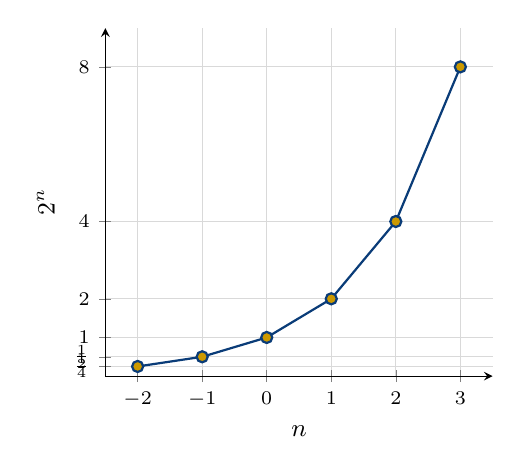
\begin{tikzpicture}
      \begin{axis}[
        width=6.5cm, height=6cm,
        xlabel={$n$}, ylabel={$2^n$},
        xlabel style={font=\small},
        ylabel style={font=\small},
        xtick={-2,-1,0,1,2,3},
        ytick={0.25,0.5,1,2,4,8},
        yticklabels={$\frac{1}{4}$,$\frac{1}{2}$,$1$,$2$,$4$,$8$},
        tick label style={font=\scriptsize},
        grid=both, grid style={gray!30},
        axis lines=left,
        ymin=0, ymax=9,
        xmin=-2.5, xmax=3.5,
      ]
        \addplot[azuloscuro, thick, mark=*, mark options={fill=dorado, draw=azuloscuro}]
          coordinates {(-2,0.25) (-1,0.5) (0,1) (1,2) (2,4) (3,8)};
      \end{axis}
    \end{tikzpicture}
    \vspace{4pt}
    \begin{block}{$\star$\; Patrón detectado}
      \small Cada vez que el exponente decrece en $1$, el valor se \textbf{divide} entre la base. Este patrón \emph{define} los exponentes negativos de manera coherente.
    \end{block}
  \end{columns}
\end{frame}

% ═══════════════════════════════════════════════
\section{Propiedades de las Potencias}
% ═══════════════════════════════════════════════

\begin{frame}{Propiedades Fundamentales I}
  \begin{columns}[T]
    \column{0.48\textwidth}

    \begin{propiedad}{P1 · Producto de potencias (misma base)}
      \[a^m \cdot a^n = a^{m+n}\]
      \textit{Ejemplo:} $\;x^3 \cdot x^5 = x^8$
    \end{propiedad}
    \vspace{6pt}

    \begin{propiedad}{P2 · Cociente de potencias (misma base)}
      \[\frac{a^m}{a^n} = a^{m-n}, \quad a \neq 0\]
      \textit{Ejemplo:} $\;\dfrac{y^7}{y^3} = y^4$
    \end{propiedad}
    \vspace{6pt}

    \begin{propiedad}{P3 · Potencia de una potencia}
      \[\left(a^m\right)^n = a^{m\cdot n}\]
      \textit{Ejemplo:} $\;\left(z^2\right)^5 = z^{10}$
    \end{propiedad}

    \column{0.48\textwidth}

    \begin{propiedad}{P4 · Potencia de un producto}
      \[(ab)^n = a^n \cdot b^n\]
      \textit{Ejemplo:} $\;(2x)^3 = 8x^3$
    \end{propiedad}
    \vspace{6pt}

    \begin{propiedad}{P5 · Potencia de un cociente}
      \[\left(\frac{a}{b}\right)^n = \frac{a^n}{b^n}, \quad b \neq 0\]
      \textit{Ejemplo:} $\;\left(\dfrac{x}{3}\right)^2 = \dfrac{x^2}{9}$
    \end{propiedad}
    \vspace{6pt}

    \begin{alerta_box}{Errores frecuentes}
      \small $\bullet\; (a+b)^2 \neq a^2+b^2$\\
      $\bullet\; a^m \cdot b^n \neq (ab)^{m+n}$ (bases distintas)
    \end{alerta_box}

  \end{columns}
\end{frame}

\begin{frame}{Demostración: Propiedad P1}
  \begin{block}{Demostración de $a^m \cdot a^n = a^{m+n}$}
    \[
      a^m \cdot a^n
      = \underbrace{(a \cdot a \cdots a)}_{m}\cdot \underbrace{(a \cdot a \cdots a)}_{n}
      = \underbrace{a \cdot a \cdots a}_{m+n}
      = a^{m+n} \qquad \square
    \]
  \end{block}

  \vspace{8pt}

  \begin{ejercicio}{Aplicación escalonada de propiedades}
    Simplifica completamente: $\;\dfrac{\left(2x^3\right)^4 \cdot x^{-2}}{8x^5}$

    \medskip
    \textbf{Solución paso a paso:}
    \begin{align*}
      \frac{\left(2x^3\right)^4 \cdot x^{-2}}{8x^5}
      &= \frac{2^4 \cdot x^{12} \cdot x^{-2}}{8x^5}
        && \text{(P4)} \\[4pt]
      &= \frac{16 \cdot x^{10}}{8x^5}
        && \text{(P1)} \\[4pt]
      &= 2x^{10-5}
        && \text{(P2)} \\[4pt]
      &= \boxed{2x^5}
    \end{align*}
  \end{ejercicio}
\end{frame}

\begin{frame}{Notación Científica: Potencias en Contexto}
  \begin{columns}[T]
    \column{0.5\textwidth}
    \begin{definicion}{Notación Científica}
      Un número real $N$ está en notación científica si:
      \[
        N = a \times 10^n, \quad 1 \leq |a| < 10,\; n \in \mathbb{Z}
      \]
    \end{definicion}
    \vspace{6pt}
    \begin{block}{Ejemplos del mundo real}
      \small
      \renewcommand{\arraystretch}{1.3}
      \begin{tabular}{lc}
        \toprule
        Magnitud & Valor \\
        \midrule
        Masa del electrón & $9.109 \times 10^{-31}$ kg \\
        Distancia Tierra-Sol & $1.496 \times 10^{11}$ m \\
        Población mundial & $8.1 \times 10^{9}$ hab \\
        Constante de Avogadro & $6.022 \times 10^{23}$ \\
        \bottomrule
      \end{tabular}
    \end{block}

    \column{0.46\textwidth}
    \begin{ejercicio}{Operaciones en notación científica}
      \small Calcula:
      \[
        \frac{(3 \times 10^4)(2 \times 10^{-7})}{6 \times 10^{-5}}
      \]
      \textbf{Solución:}
      \begin{align*}
        &= \frac{3 \cdot 2}{6} \times \frac{10^{4} \cdot 10^{-7}}{10^{-5}}\\[4pt]
        &= 1 \times 10^{4+(-7)-(-5)}\\[4pt]
        &= 1 \times 10^{2}\\[4pt]
        &= \boxed{100}
      \end{align*}
    \end{ejercicio}
    \begin{alerta_box}{Verificación}
      Siempre verifica que el coeficiente del resultado esté en $[1,10)$.
    \end{alerta_box}
  \end{columns}
\end{frame}

% ═══════════════════════════════════════════════
\section{Álgebra en los Reales}
% ═══════════════════════════════════════════════

\begin{frame}{Elementos del Álgebra: Términos y Expresiones}
  \begin{columns}[T]
    \column{0.5\textwidth}
    \begin{definicion}{Término algebraico}
      Un \textbf{término algebraico} es un producto de un coeficiente numérico y una o más variables elevadas a potencias no negativas:
      \[
        \underbrace{-5}_{\text{coeficiente}}\;\underbrace{x^3 y^2}_{\text{parte literal}}
      \]
    \end{definicion}
    \vspace{6pt}
    \begin{definicion}{Expresión algebraica}
      Una \textbf{expresión algebraica} es una combinación de términos mediante operaciones aritméticas:
      \[
        3x^2 - 7xy + 4y^2 - 1
      \]
      Esta expresión tiene \textbf{4 términos}.
    \end{definicion}

    \column{0.46\textwidth}
    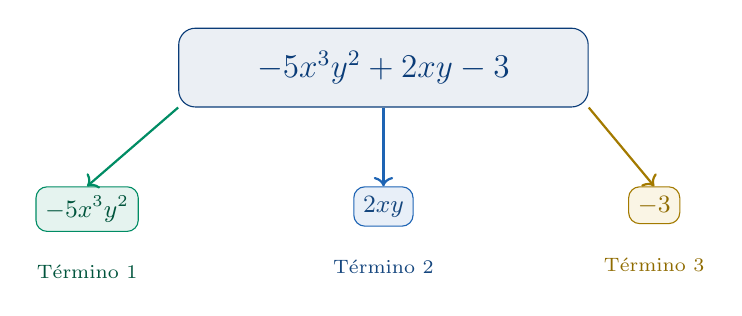
\begin{tikzpicture}[scale=0.9, every node/.style={font=\small}]
      \node[draw=azuloscuro, fill=azuloscuro!8, rounded corners=6pt,
            minimum width=5.2cm, minimum height=1cm,
            font=\large\bfseries, text=azuloscuro] (expr) at (0,0)
            {$\;-5x^3y^2 + 2xy - 3\;$};

      \node[draw=verdeclaro, fill=verdeclaro!10, rounded corners=4pt,
            text=verdeclaro!60!black, font=\small\bfseries,
            below left=1cm and 0.5cm of expr] (t1)
            {$-5x^3y^2$};
      \node[draw=azulmedio, fill=azulmedio!10, rounded corners=4pt,
            text=azulmedio!70!black, font=\small\bfseries,
            below=1cm of expr] (t2) {$2xy$};
      \node[draw=dorado!80!black, fill=dorado!10, rounded corners=4pt,
            text=dorado!70!black, font=\small\bfseries,
            below right=1cm and 0.5cm of expr] (t3) {$-3$};

      \draw[->, verdeclaro, thick] (expr.south west) -- (t1.north);
      \draw[->, azulmedio, thick]  (expr.south) -- (t2.north);
      \draw[->, dorado!80!black, thick] (expr.south east) -- (t3.north);

      \node[below=0.3cm of t1, font=\scriptsize, text=verdeclaro!60!black] {Término 1};
      \node[below=0.3cm of t2, font=\scriptsize, text=azulmedio!70!black] {Término 2};
      \node[below=0.3cm of t3, font=\scriptsize, text=dorado!70!black] {Término 3};
    \end{tikzpicture}

    \vspace{6pt}
    \begin{block}{$\blacksquare$\; Vocabulario clave}
      \small
      \textbf{Monomio}: 1 término \quad \textbf{Binomio}: 2 términos\\
      \textbf{Trinomio}: 3 términos \quad \textbf{Polinomio}: $n$ términos
    \end{block}
  \end{columns}
\end{frame}

\begin{frame}{Términos Semejantes}
  \begin{columns}[T]
    \column{0.48\textwidth}
    \begin{definicion}{Términos semejantes}
      Dos o más términos son \textbf{semejantes} si tienen \emph{exactamente la misma parte literal} (mismas variables con los mismos exponentes).
    \end{definicion}
    \vspace{6pt}

    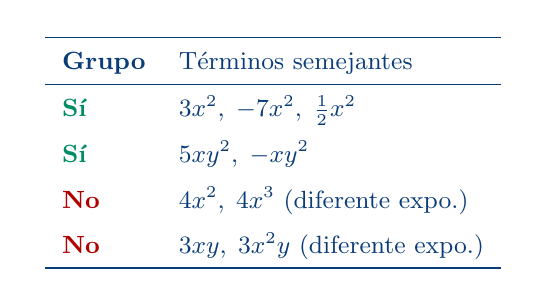
\begin{tikzpicture}
      \node[font=\small, text=azuloscuro] at (0,0) {
        \renewcommand{\arraystretch}{1.5}
        \begin{tabular}{>{\bfseries}l l}
          \hline
          Grupo & Términos semejantes \\
          \hline
          \textcolor{verdeclaro}{Sí} & $3x^2,\;-7x^2,\; \tfrac{1}{2}x^2$ \\
          \textcolor{verdeclaro}{Sí} & $5xy^2,\; -xy^2$ \\
          \textcolor{red!70!black}{No} & $4x^2,\; 4x^3$ (diferente expo.) \\
          \textcolor{red!70!black}{No} & $3xy,\; 3x^2y$ (diferente expo.) \\
          \hline
        \end{tabular}
      };
    \end{tikzpicture}

    \column{0.48\textwidth}
    \begin{propiedad}{Reducción de términos semejantes}
      Se aplica la \textbf{propiedad distributiva}: solo se suman/restan los coeficientes, manteniendo la parte literal:
      \[
        \alpha \cdot t + \beta \cdot t = (\alpha + \beta)\cdot t
      \]
    \end{propiedad}
    \vspace{6pt}
    \begin{ejercicio}{Simplificación}
      \small
      \[
        5x^2 - 3x + 7x^2 + x - 2
      \]
      \begin{align*}
        &= (5+7)x^2 + (-3+1)x - 2\\
        &= \boxed{12x^2 - 2x - 2}
      \end{align*}
    \end{ejercicio}
  \end{columns}
\end{frame}

\begin{frame}{Grado de un Polinomio}
  \begin{columns}[T]
    \column{0.5\textwidth}
    \begin{definicion}{Grado de un término}
      El \textbf{grado} de un término es la suma de los exponentes de todas sus variables:
      \[
        \deg(c\, x_1^{a_1} x_2^{a_2} \cdots x_k^{a_k}) = \sum_{i=1}^k a_i
      \]
    \end{definicion}
    \vspace{4pt}
    \begin{block}{Ejemplos}
      \small
      \begin{itemize}[leftmargin=*]
        \item $\deg(4x^3y^2) = 3+2 = 5$
        \item $\deg(7xy) = 1+1 = 2$
        \item $\deg(-8) = 0$ (constante)
      \end{itemize}
    \end{block}

    \column{0.46\textwidth}
    \begin{definicion}{Grado de un polinomio}
      Es el \textbf{mayor grado} entre todos sus términos (reducidos).
    \end{definicion}
    \vspace{6pt}
    \begin{ejercicio}{Determinar el grado}
      \small
      \[
        P(x,y) = 3x^4 - 2x^2y^3 + xy - 5
      \]
      Grados por término: $4,\; 5,\; 2,\; 0$.\\[4pt]
      $\therefore$ $P$ tiene \textbf{grado 5}.
    \end{ejercicio}
    \vspace{6pt}
    \begin{alerta_box}{Forma canónica}
      Un polinomio en $x$ se escribe en \textbf{forma canónica} cuando sus términos están ordenados de mayor a menor grado.
    \end{alerta_box}
  \end{columns}
\end{frame}

% ═══════════════════════════════════════════════
\section{Patrones y Relaciones Algebraicas}
% ═══════════════════════════════════════════════

\begin{frame}{Detección de Patrones: Identidades Notables}
  \begin{columns}[T]
    \column{0.5\textwidth}
    \begin{propiedad}{Cuadrado de una suma}
      \[
        (a+b)^2 = a^2 + 2ab + b^2
      \]
    \end{propiedad}
    \vspace{4pt}
    \begin{propiedad}{Cuadrado de una diferencia}
      \[
        (a-b)^2 = a^2 - 2ab + b^2
      \]
    \end{propiedad}
    \vspace{4pt}
    \begin{propiedad}{Diferencia de cuadrados}
      \[
        (a+b)(a-b) = a^2 - b^2
      \]
    \end{propiedad}
    \vspace{4pt}
    \begin{propiedad}{Cubo de una suma}
      \[
        (a+b)^3 = a^3 + 3a^2b + 3ab^2 + b^3
      \]
    \end{propiedad}

    \column{0.46\textwidth}
    \textbf{\color{azuloscuro}Verificación geométrica: $(a+b)^2$}
    \vspace{8pt}

    \begin{tikzpicture}[scale=0.85]
      \def\a{2.4} \def\b{1.2}

      % Big square
      \draw[thick, azuloscuro, fill=azuloscuro!5] (0,0) rectangle (\a+\b,\a+\b);

      % Inner squares and rectangles
      \fill[azulmedio!30] (0,\b) rectangle (\a,\a+\b); % a^2
      \fill[dorado!30] (\a,0) rectangle (\a+\b,\b);    % b^2
      \fill[verdeclaro!30] (0,0) rectangle (\a,\b);    % ab
      \fill[verdeclaro!30] (\a,\b) rectangle (\a+\b,\a+\b); % ab

      % Labels inside
      \node[font=\small\bfseries, text=azulmedio!80!black] at (\a/2,(\b+\a+\b)/2) {$a^2$};
      \node[font=\small\bfseries, text=dorado!80!black] at (\a+\b/2,\b/2) {$b^2$};
      \node[font=\small, text=verdeclaro!60!black] at (\a/2,\b/2) {$ab$};
      \node[font=\small, text=verdeclaro!60!black] at (\a+\b/2,(\b+\a+\b)/2) {$ab$};

      % Dimension labels
      \draw[<->, thick, azuloscuro] (0,-0.3)--(\a,-0.3) node[midway,below,font=\small]{$a$};
      \draw[<->, thick, azuloscuro] (\a,-0.3)--(\a+\b,-0.3) node[midway,below,font=\small]{$b$};
      \draw[<->, thick, azuloscuro] (-0.3,0)--(-0.3,\b) node[midway,left,font=\small]{$b$};
      \draw[<->, thick, azuloscuro] (-0.3,\b)--(-0.3,\a+\b) node[midway,left,font=\small]{$a$};
    \end{tikzpicture}

    \vspace{4pt}
    \[
      \textcolor{azuloscuro}{(a+b)^2} = \textcolor{azulmedio!80!black}{a^2} + \textcolor{verdeclaro!60!black}{ab} + \textcolor{verdeclaro!60!black}{ab} + \textcolor{dorado!80!black}{b^2}
    \]
  \end{columns}
\end{frame}

\begin{frame}{Patrones en el Triángulo de Pascal y el Binomio de Newton}
  \begin{columns}[T]
    \column{0.45\textwidth}
    \textbf{\color{azuloscuro}Triángulo de Pascal:}
    \vspace{6pt}

    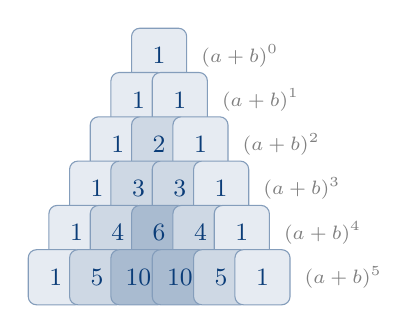
\begin{tikzpicture}[scale=0.75, every node/.style={font=\small},
      nd/.style={draw=azuloscuro!50, fill=azuloscuro!10, rounded corners=3pt,
                 minimum size=0.7cm, text=azuloscuro}]
      % Row 0
      \node[nd] at (0,0) {1};
      \node[right=0.15cm,font=\scriptsize\itshape,text=gray] at (0.35,0) {$(a+b)^0$};
      % Row 1
      \node[nd] at (-0.35,-0.75) {1}; \node[nd] at (0.35,-0.75) {1};
      \node[right=0.15cm,font=\scriptsize\itshape,text=gray] at (0.7,-0.75) {$(a+b)^1$};
      % Row 2
      \node[nd] at (-0.7,-1.5) {1}; \node[nd,fill=azuloscuro!20] at (0,-1.5) {2}; \node[nd] at (0.7,-1.5) {1};
      \node[right=0.15cm,font=\scriptsize\itshape,text=gray] at (1.05,-1.5) {$(a+b)^2$};
      % Row 3
      \node[nd] at (-1.05,-2.25) {1}; \node[nd,fill=azuloscuro!20] at (-0.35,-2.25) {3};
      \node[nd,fill=azuloscuro!20] at (0.35,-2.25) {3}; \node[nd] at (1.05,-2.25) {1};
      \node[right=0.15cm,font=\scriptsize\itshape,text=gray] at (1.4,-2.25) {$(a+b)^3$};
      % Row 4
      \node[nd] at (-1.4,-3) {1}; \node[nd,fill=azuloscuro!20] at (-0.7,-3) {4};
      \node[nd,fill=azuloscuro!35] at (0,-3) {6};
      \node[nd,fill=azuloscuro!20] at (0.7,-3) {4}; \node[nd] at (1.4,-3) {1};
      \node[right=0.15cm,font=\scriptsize\itshape,text=gray] at (1.75,-3) {$(a+b)^4$};
      % Row 5
      \node[nd] at (-1.75,-3.75) {1}; \node[nd,fill=azuloscuro!20] at (-1.05,-3.75) {5};
      \node[nd,fill=azuloscuro!35] at (-0.35,-3.75) {10};
      \node[nd,fill=azuloscuro!35] at (0.35,-3.75) {10};
      \node[nd,fill=azuloscuro!20] at (1.05,-3.75) {5}; \node[nd] at (1.75,-3.75) {1};
      \node[right=0.15cm,font=\scriptsize\itshape,text=gray] at (2.1,-3.75) {$(a+b)^5$};
    \end{tikzpicture}

    \column{0.52\textwidth}
    \begin{propiedad}{Teorema del Binomio de Newton}
      \[
        (a+b)^n = \sum_{k=0}^{n} \binom{n}{k} a^{n-k}b^k
      \]
      donde $\dbinom{n}{k} = \dfrac{n!}{k!(n-k)!}$
    \end{propiedad}
    \vspace{6pt}
    \begin{ejercicio}{Expansión usando el Binomio}
      \small Expande $(x - 2)^4$:
      \begin{align*}
        &= \binom{4}{0}x^4(-2)^0 + \binom{4}{1}x^3(-2)^1\\
        &\quad+ \binom{4}{2}x^2(-2)^2 + \binom{4}{3}x(-2)^3\\
        &\quad+ \binom{4}{4}(-2)^4\\
        &= \boxed{x^4 - 8x^3 + 24x^2 - 32x + 16}
      \end{align*}
    \end{ejercicio}
  \end{columns}
\end{frame}

\begin{frame}{Relaciones e Inconsistencias: Análisis Crítico}
  \begin{columns}[T]
    \column{0.5\textwidth}
    \begin{alerta_box}{Inconsistencia 1: ``Cancelación'' indebida}
      \small
      \textbf{Afirmación falsa:}
      \[
        \frac{x^2 - 4}{x-2} = x+2 \quad \forall x
      \]
      \textbf{Error:} La expresión \emph{no está definida} para $x=2$.\\[4pt]
      \textbf{Correcto:}
      \[
        \frac{x^2-4}{x-2} = x+2, \quad x \neq 2
      \]
    \end{alerta_box}
    \vspace{6pt}
    \begin{alerta_box}{Inconsistencia 2: Potencia de suma}
      \small
      \textbf{Afirmación falsa:}
      \[
        (3+5)^2 \stackrel{?}{=} 3^2 + 5^2 = 34
      \]
      \textbf{Correcto:} $(3+5)^2 = 8^2 = 64$\\
      El término cruzado $2\cdot3\cdot5=30$ no fue omitido.
    \end{alerta_box}

    \column{0.46\textwidth}
    \begin{block}{$\circ$\; Estrategia: detección de errores}
      \small
      Para verificar una identidad algebraica, aplica el \textbf{método de sustitución numérica}: reemplaza valores específicos.\\[6pt]
      Si la igualdad falla para \emph{un} valor, es \textbf{falsa}.\\
      Si se verifica para \emph{todos}, considerar demostración formal.
    \end{block}
    \vspace{6pt}
    \begin{ejercicio}{Detecta el error}
      \small Analiza si la siguiente simplificación es válida:
      \[
        \frac{a^2}{a} \stackrel{?}{=} a \quad \forall a \in \mathbb{R}
      \]
      \textit{¿Para qué valores falla? ¿Por qué?}\\[4pt]
      \textbf{Respuesta:} Falla en $a = 0$ (división por cero). La igualdad es válida \emph{solo} para $a \neq 0$.
    \end{ejercicio}
  \end{columns}
\end{frame}

\begin{frame}{Integración: Patrones en Sucesiones y Polinomios}
  \begin{columns}[T]
    \column{0.5\textwidth}
    \begin{block}{Sucesión de cuadrados perfectos}
      \small
      \[
        1,\; 4,\; 9,\; 16,\; 25,\; \ldots
      \]
      El \textbf{patrón}: $a_n = n^2$\\[4pt]
      \textbf{Diferencias sucesivas} (1er orden): $3, 5, 7, 9, \ldots$\\
      \textbf{Diferencias} (2do orden): $2, 2, 2, \ldots$ (\emph{constante})\\[4pt]
      $\star$\; Un polinomio de grado $k$ tiene diferencias \textbf{finitas de orden $k$} constantes. Este es un resultado fundamental del cálculo en diferencias finitas.
    \end{block}
    \vspace{6pt}
    \begin{ejercicio}{Identifica el grado}
      \small La sucesión $1, 8, 27, 64, 125, \ldots$ corresponde a $n^3$. Verifica que sus diferencias de orden 3 son constantes.
    \end{ejercicio}

    \column{0.46\textwidth}
    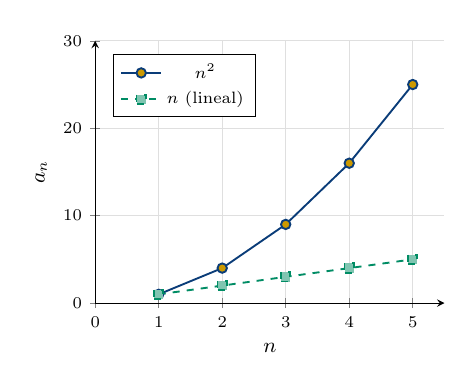
\begin{tikzpicture}[scale=0.85]
      \begin{axis}[
        width=6.8cm, height=5.5cm,
        xlabel={$n$}, ylabel={$a_n$},
        xlabel style={font=\small},
        ylabel style={font=\small},
        tick label style={font=\scriptsize},
        grid=both, grid style={gray!25},
        axis lines=left,
        ymin=0, ymax=30,
        xmin=0, xmax=5.5,
        legend style={font=\scriptsize, at={(0.05,0.95)}, anchor=north west}
      ]
        \addplot[azuloscuro, thick, mark=*, mark options={fill=dorado}]
          coordinates {(1,1)(2,4)(3,9)(4,16)(5,25)};
        \addlegendentry{$n^2$}
        \addplot[verdeclaro, thick, dashed, mark=square*, mark options={fill=verdeclaro!50}]
          coordinates {(1,1)(2,2)(3,3)(4,4)(5,5)};
        \addlegendentry{$n$ (lineal)}
      \end{axis}
    \end{tikzpicture}
    \vspace{4pt}
    \begin{block}{$\nearrow$\; Relación clave}
      \small El comportamiento \textbf{cuadrático} de $n^2$ vs el \textbf{lineal} de $n$ ilustra cómo el exponente determina la tasa de crecimiento.
    \end{block}
  \end{columns}
\end{frame}

% ═══════════════════════════════════════════════
%  EJERCICIOS INTEGRADORES
% ═══════════════════════════════════════════════

\begin{frame}{Ejercicios Integradores}
  \begin{columns}[T]
    \column{0.48\textwidth}
    \begin{ejercicio}{Nivel I — Propiedades}
      \small Simplifica cada expresión:
      \begin{enumerate}[label=\textbf{\alph*.}]
        \item $\dfrac{(x^2 y)^3 \cdot x^{-1}}{x^4 y^2}$
        \item $(2a^3 b^{-2})^2 \cdot (ab)^{-1}$
        \item $\dfrac{3^{n+2} - 3^n}{3^n}$
      \end{enumerate}
    \end{ejercicio}
    \vspace{6pt}
    \begin{ejercicio}{Nivel II — Términos semejantes}
      \small Reduce y clasifica el polinomio resultante:
      \[
        (3x^2 - 2x + 1) + (x^2 + 5x - 4) - (x^2 - x + 2)
      \]
    \end{ejercicio}

    \column{0.48\textwidth}
    \begin{ejercicio}{Nivel III — Identidades}
      \small
      \begin{enumerate}[label=\textbf{\alph*.}]
        \item Expande y simplifica:\\
          $(2x-3)^2 + (2x+3)^2$
        \item Factoriza usando identidades:\\
          $9a^4 - 24a^2b + 16b^2$
        \item Demuestra algebraicamente:\\
          $(x+y)^3 - (x-y)^3 = 2y(3x^2+y^2)$
      \end{enumerate}
    \end{ejercicio}
    \vspace{6pt}
    \begin{ejercicio}{Nivel IV — Detección de patrones}
      \small Dada la sucesión $P(n) = 2n^2 - n + 3$, calcula $P(1),\ldots, P(5)$, construye las diferencias finitas y verifica que son de grado 2.
    \end{ejercicio}
  \end{columns}
\end{frame}

% ═══════════════════════════════════════════════
%  CIERRE
% ═══════════════════════════════════════════════

\begin{frame}{Síntesis de la Sesión}
  \begin{columns}[T]
    \column{0.5\textwidth}
    \begin{block}{\checkmark\; Lo que aprendimos hoy}
      \small
      \begin{itemize}[leftmargin=*]
        \item[\textcolor{verdeclaro}{\checkmarkCircle}] \textbf{Potencia} como producto iterado: $a^n$
        \item[\textcolor{verdeclaro}{\checkmarkCircle}] \textbf{Propiedades} P1–P5 y exponentes negativos
        \item[\textcolor{verdeclaro}{\checkmarkCircle}] \textbf{Término} y \textbf{expresión algebraica}; grado de polinomio
        \item[\textcolor{verdeclaro}{\checkmarkCircle}] \textbf{Términos semejantes}: reducción por distributividad
        \item[\textcolor{verdeclaro}{\checkmarkCircle}] \textbf{Identidades notables} como patrones algebraicos
        \item[\textcolor{verdeclaro}{\checkmarkCircle}] \textbf{Detección de errores} e inconsistencias típicas
      \end{itemize}
    \end{block}

    \column{0.46\textwidth}
    \begin{block}{$\bullet$\; Mapa conceptual}
      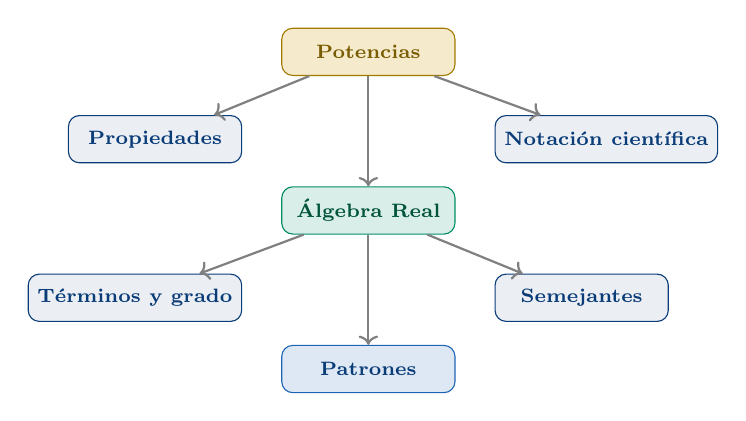
\begin{tikzpicture}[
          scale=0.75,
          node distance=0.7cm,
          box/.style={draw=azuloscuro, fill=azuloscuro!8, rounded corners=4pt,
                      font=\scriptsize\bfseries, text=azuloscuro,
                      minimum width=2.2cm, minimum height=0.6cm}
        ]
        \node[box, fill=dorado!20, draw=dorado!80!black, text=dorado!60!black] (pot) {Potencias};
        \node[box, below left=of pot] (prop) {Propiedades};
        \node[box, below right=of pot] (notc) {Notación científica};
        \node[box, below=1.4cm of pot, fill=verdeclaro!15, draw=verdeclaro, text=verdeclaro!60!black] (alg) {Álgebra Real};
        \node[box, below left=of alg] (term) {Términos y grado};
        \node[box, below right=of alg] (sem) {Semejantes};
        \node[box, below=1.4cm of alg, fill=azulmedio!15, draw=azulmedio] (pat) {Patrones};
        \draw[->, thick, gray] (pot)--(prop);
        \draw[->, thick, gray] (pot)--(notc);
        \draw[->, thick, gray] (pot)--(alg);
        \draw[->, thick, gray] (alg)--(term);
        \draw[->, thick, gray] (alg)--(sem);
        \draw[->, thick, gray] (alg)--(pat);
      \end{tikzpicture}
    \end{block}
  \end{columns}

  \vspace{8pt}
  \begin{center}
    
\begin{tikzpicture}
      \node[draw=dorado, fill=dorado!15, rounded corners=6pt,
            font=\small\itshape, text=dorado!70!black,
            inner xsep=12pt, inner ysep=6pt]
        {``El álgebra es el lenguaje que usa la matemática para revelar los patrones ocultos del universo.''};
    \end{tikzpicture}
  \end{center}
\end{frame}

\begin{frame}{Tarea y Lecturas Complementarias}
  \begin{columns}[T]
    \column{0.5\textwidth}
    \begin{block}{\ding{46}\; Para la próxima sesión}
      \small
      \begin{enumerate}[leftmargin=*]
        \item Demostrar formalmente las propiedades P3, P4 y P5 a partir de la definición.
        \item Resolver los ejercicios integradores de la diapositiva anterior (mostrar procedimiento completo).
        \item Investigar la conexión entre el Triángulo de Pascal y las combinaciones $\binom{n}{k}$.
        \item Proponer un ejemplo propio de una ``inconsistencia'' algebraica frecuente y su corrección.
      \end{enumerate}
    \end{block}

    \column{0.46\textwidth}
    \begin{block}{$\bullet$\; Bibliografía}
      \small
      \begin{itemize}[leftmargin=*]
        \item Stewart, J. (2018). \textit{Precálculo: Matemáticas para el Cálculo}, 7.ª ed. Cengage.
        \item Apostol, T. (2006). \textit{Calculus}, Vol. 1, 2.ª ed. Wiley.
        \item Lay, D. et al. (2016). \textit{Álgebra Lineal y sus Aplicaciones}, 5.ª ed. Pearson.
        \item Spivak, M. (2008). \textit{Calculus}, 4th ed. Publish or Perish.
      \end{itemize}
    \end{block}
    \vspace{6pt}
    \begin{center}
      \large\textbf{\color{azuloscuro}¿Preguntas?}\\[4pt]
      \small\color{gray}$\bullet$\; catedra.matematicas@universidad.cl
    \end{center}
  \end{columns}
\end{frame}

\end{document}
